\documentclass[10pt,a4paper]{article}
\usepackage[utf8]{inputenc}
%\usepackage[german]{babel}
%\usepackage[cyrillic]{babel}
\usepackage[T1]{fontenc}
\usepackage{amsmath}
\usepackage{amsfonts}
\usepackage{amssymb}
\usepackage{amsthm}

%\renewcommand{\thesubsection}{\arabic{subsection}}
%\newtheorem{thm}{Theorem}[section]
%\renewcommand{\thethm}{\arabic{subsection}.\arabic{thm}}

\usepackage{thmtools}
\usepackage{hyperref}
\hypersetup{
    colorlinks=true,
    linkcolor=blue,
    filecolor=magenta,      
    urlcolor=cyan,
    pdftitle={Overleaf Example},
    %pdfpagemode=FullScreen,
    }
%\usepackage{stix-type1}%\turnediota
\theoremstyle{definition}

\newtheorem{constructor}{Constructor}[section]
\newtheorem{axiom}{Axiom}
\newtheorem{definition}{Definition}[section]
\newtheorem{lemma}{Lemma}[section]
\newtheorem{theorem}{Theorem}[section]
\newtheorem{note}{Note}[section]
\usepackage{etoolbox}

%\newcommand*{\@Dashv}[2]{%
%  \reflectbox{$\m@th#1#2$}%
%}
\newcommand*{\separation}[3]{% 1)binder, 2)set, 3)condition
  \{#1\in #2: #3\}
}

% https://www.freecodecamp.org/news/simple-regex-tricks-for-beginners-3acb3fa257cb/
%  \\mathcal\{T\} |---> \topology
%  \\mathcal\{([^\}]*)\}   |--->  $1
\newcommand{\AND}{\ \ \&\ \ }
\newcommand{\borel}{\mathcal{B}}
\newcommand{\closure}{\mbox{cl}}
\newcommand{\complex}{\mathbb{C}}
\newcommand{\converges}{\longrightarrow}
\newcommand{\countable}{\mbox{\ countable}}
\newcommand{\defined}{\mbox{\ defined}}
\newcommand{\dom}{\mbox{dom}}
\newcommand{\Done}{\noindent \textbf{Done.}\\}
\newcommand{\function}{\mathrm{\ function}}
\newcommand{\functional}{\mbox{\ functional}}
\newcommand{\IFF}{\ \Longleftrightarrow\ }
\renewcommand{\iff}{\ \longleftrightarrow\ }
\newcommand{\IMPLIES}{\ \Longrightarrow\ }
\renewcommand{\implies}{\ \longrightarrow\ }
\newcommand{\Inf}{\mathrm{Inf}}
\newcommand{\injective}{\mbox{\ injective}}
\newcommand{\injection}{\mbox{\ injection}}
\newcommand{\interior}{\mbox{int}}
\newcommand{\intersection}{\bigcap}
\newcommand{\isempty}{\mathrm{\ empty}}
\newcommand{\LB}{\mathrm{LB}}
\newcommand{\nghbset}{\mathcal{N}}
\newcommand{\nonempty}{\mathrm{\ nonempty}}
\newcommand{\power}{\mathcal{P}}
\newcommand{\Proof}{\noindent \textbf{Proof.}\\}
\newcommand{\real}{\mathbb{R}}
\newcommand{\relation}{\mathrm{\ relation}}
\newcommand{\set}{\mathrm{\ set}}
\newcommand{\singleton}{\mathrm{\ singleton}}
\newcommand{\semialgebra}{\mathcal{S}}
\newcommand{\Sup}{\mathrm{Sup}}
\newcommand{\surjective}{\mbox{\ surjective\ on\ }}
\newcommand{\Term}{\mathrm{Term}}
\newcommand{\topology}{\mathcal{T}}
\newcommand{\total}{\mbox{\ total\ on\ }}
\newcommand{\transitive}{\mathrm{\ transitive}}
\newcommand{\union}{\bigcup}
\newcommand{\univocal}{\mathrm{\ univocal}}
\newcommand{\univocalat}{\mathrm{\ univocal\ at\ }}
\newcommand{\UB}{\mathrm{UB}}
\newcommand{\Var}{\mathrm{Var}}

\newcommand{\notvarphi}{\phi}
\renewcommand{\phi}{\varphi}

\newcommand{\comment}[1]{\quad\mbox{(#1)}}
% local commands
%\preto\section{\undef\blipo} %etoolbox
\preto\subsection{\undef\blipo} %etoolbox
% https://tex.stackexchange.com/questions/105684/limit-macro-newcommand-scope-to-section
\usepackage{graphicx}
\usepackage{authblk}
\title{Formalisation of theorems}
\author[1]{Georgy Dunaev}
\begin{document}
\maketitle
\begin{center}
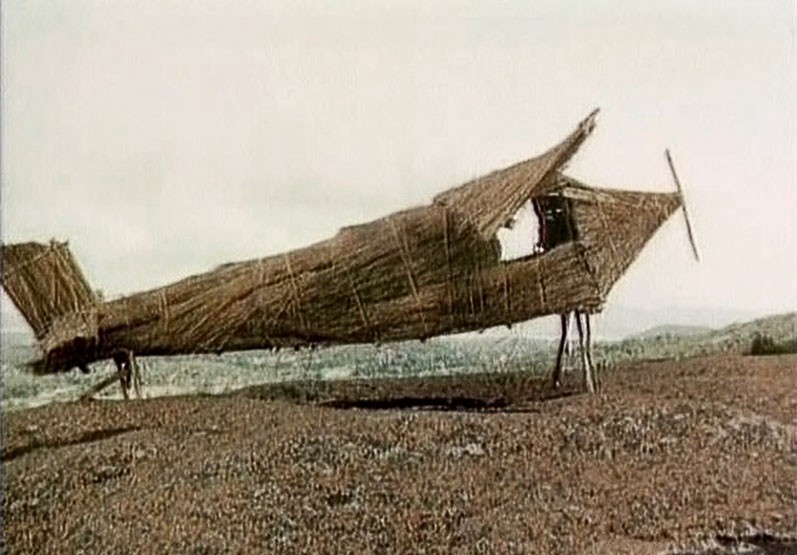
\includegraphics[scale=0.5]{cargo.jpeg}
\end{center}
\thispagestyle{empty}
\pagebreak
\newpage
\ \\
\thispagestyle{empty}
\pagebreak
\newpage
\pagebreak
\newpage

\tableofcontents
\newpage
%qwertyuio
\noindent
% of functional analysis and topology. It is needed because writing it by hand leads to severe amount of corrections, while implementing it with an interactive proof assistant is tedious and platform-dependent.\\
%\noindent
% elements are small letters, sets are uppercase latin letters, sets of sets are mathcal latin letters
% the code should be comprehensive: use meaning ozf symbols
Motivation: there are lots of proof assistants which allow to prove mathematical theorems, but their use for the purposes of an average mathematician is deeply disappointing due to various reasons.\\

I am creating a proof assistant and this document is a very early prologue to what the computer-generated article will look like.\\

The other point of creating such document is to provide programmed classical logical foundations for developing a set-theoretic proofs, and vice-versa to provide a set-theoretic foundations to prove theorems about logic.
\noindent
\subsection{Goals}
%Interesting targets:
\begin{itemize}
\item The aim of this document is to provide standard classical mathematical foundations as well as some amount of perfect proofs.
\item The proof assistant based on this very classical theory is being implemented. \url{https://github.com/georgydunaev/set_theory_prover}
\item After completion of development of the program, not only tactics, but also machine learning algorithms may be applied in a search of the proofs.

%\item sequential criterion
%\item completion of a metric space
\end{itemize}
%...
\newpage
\section{Foundations [skip this section; go to section 3]}
\subsection{Basic definitions}
...
\begin{definition} Simultaneous substitution.
\[
\varphi[Z_1/W_1,...,Z_n/W_n]
\]
\end{definition}
\noindent
...
\subsection{Useful metatheorems}
\begin{theorem}
\[
A=B\ \Longrightarrow\ (t[A/W]=t[B/W])
\]
\end{theorem}
\Proof
Assume $A=B$.
By induction on term construction.\\
Case 1(Base): $t=v\in \Var$\\
If also the variable $v$ is $W$ then $t[A/W]=A$ and $t[B/W]=B$.\\
Since $A=B$, $t[A/W]=t[B/W]$, so we are done.
Otherwise, i.e. if the variable $v$ is not $W$, then $t[A/W]=v=t$ and $t[B/W]=v=t$.\\
Therefore $t[A/W]=t[B/W]$, so we are done.\\
Case 2(Step of induction): $t=f(t_1,...,t_n)\in\Term$, where $f$ is a functional symbol of arity n.\\
Now we can use induction hypotheses: $t_1[A/W]=t_1[B/W],...,t_n[A/W]=t_n[B/W]$ and definition of substitution.
\[
t[A/W]=f(t_1,...,t_n)[A/W]=
\]
\[
=f(t_1[A/W],...,t_n[A/W])=
\]
\[
=f(t_1[B/W],...,t_n[B/W])=
\]
\[
=f(t_1,...,t_n)[B/W]=t[B/W]
\]
Therefore $t[A/W]=t[B/W]$, so we are done.\\
\Done

\begin{theorem}
\[
A=B
\implies
(\varphi[A/W]\ \Longleftrightarrow\ \varphi[B/W])
\]
\end{theorem}
\Proof
By induction on formula construction.\\
...\\
\Done

\subsection{Extension by definitions}
...
\pagebreak
\section{First-order logic[skip this section; go to sect.3]}
...
\begin{theorem}
\label{thm:ILMorgan}
In intuitionistic logic:\\
$\neg (A\lor B) \implies (\neg A\land\neg B)$
\end{theorem}
\Proof
Using deduction theorem it is enought to show (backward reasoning):\\
$\neg (A\lor B) \vdash (\neg A\land\neg B)$ (by OR-elim).\\
Subgoal 1: $\neg (A\lor B) \vdash \neg A$ (by deduction)\\
$\neg (A\lor B), A \vdash \bot$ (by MP $(A\lor B)\implies\bot$)\\
$\neg (A\lor B), A \vdash (A\lor B)$ (by OR-intro)\\
$\neg (A\lor B), A \vdash A$ (by assumption).\\
Subgoal 2: $\neg (A\lor B) \vdash \neg B$ (by deduction).\\
$\neg (A\lor B), B \vdash \bot$ (by MP $(A\lor B)\implies\bot$).\\
$\neg (A\lor B), B \vdash (A\lor B)$(OR-intro).\\
$\neg (A\lor B), B \vdash B$ (by assumption).\\
\Done

\begin{theorem} In intuitionistic logic:\\
\label{double neg LEM}
$\neg\neg (P\lor\neg P)$
\end{theorem}
\Proof
Using deduction theorem it is enought to show (backward reasoning):\\
$\neg (P\lor\neg P) \vdash \bot$ (cut rule with \ref{thm:ILMorgan})\\
$\neg P\land\neg\neg P \vdash \bot$ (by Left\_AND\_Intro)\\
$\neg P, \neg\neg P \vdash \bot$ (by MP: $\neg P \implies \bot$).\\
$\neg P, \neg\neg P \vdash \neg P$ (by assumption).\\
\Done

\begin{theorem}
\[
(\exists x \forall y:\varphi) \longrightarrow (\forall y \exists x :\varphi)
\]
\end{theorem}
\Proof
...\\
\Done
...
\pagebreak
\section{Class theory}%Developing set-theoretic foundations}
\begin{constructor} Subclass predicate.\\
If $A$ and $B$ are classes, then $(A\in B)$ is a formula.
\end{constructor}

%\subsection{Example of a proof (MORSE-KELLEY SET THEORY, CLASSICAL SEMANTICS)}
%\begin{constructor}
%If $\varphi$ is a formula without class-quantifiers, then
%$\{x|\varphi\}$ is NBG-class.
%\end{constructor}

%\begin{constructor}
%If $\varphi$ is a formula, then
%$\{x|\varphi\}$ is MK-class.
%\end{constructor}

\begin{constructor} Subclass predicate.\\
If $A$ and $B$ are classes, then $(A\subseteq B)$ is a formula.
\end{constructor}
\begin{definition}
\label{def:subclass}
Subclass predicate.
\[
(A\subseteq B)\iff(\forall x\in A:x\in B)
\]
\end{definition}
\begin{theorem}
\label{thm:element of subset}
\[
(x\in A)\land(A\subseteq B)\implies(x\in B)
\]
\end{theorem}
\Proof
\[
(A\subseteq B)
\IMPLIES
(\forall x\in A:x\in B)
\]
\[
(x\in A)
\AND
(\forall x\in A:x\in B)
\IMPLIES
(x\in B)
\]
\Done

If the variant of logic being used doesn't have equality, then add the following constructor and definition.
\begin{constructor}Equality.\\
If $A$ and $B$ are classes, then $(A=B)$ is a formula.
\end{constructor}
\begin{definition}
Equality. (in case if the 1st order logic is given without equality)
\[
(A=B)\iff (\forall Y: A\in Y \iff B\in Y)
\]
\end{definition}
\subsection{Axiom of extensionality}
\begin{axiom}
\label{axm:extensionality}
Extensionality.
\[
(A=B)\iff ((A\subseteq B) \land (B\subseteq A))
\]
\end{axiom}
\begin{constructor} Set predicate.\\
If $A$ is a class, then $(A\set)$ is a formula.
\end{constructor}
\begin{definition} Set predicate.
\[
(X\set)\iff(\exists Y:X\in Y)
\]
\end{definition}
\begin{theorem}
\[
(A \subseteq B)\land (B\subseteq A) \implies (A=B)
\]
\end{theorem}
\Proof
Claim: $(\forall x:x\in A \iff x\in B)$.\\
Fix x.\\
$(\Rightarrow)$\\
Assume $(x\in A)$. To show: $(x\in B)$\\
\[
(x\in A)
\AND
(A\subseteq B)
\IMPLIES
(x\in B)
\comment{by thm \ref{thm:element of subset}}
\]
$(\Leftarrow)$\\
Assume $(x\in B)$. To show: $(x\in A)$\\
\[
(x\in B)
\AND
(B\subseteq A)
\IMPLIES
(x\in A)
\comment{by thm \ref{thm:element of subset}}
\]
Claim is proven.
\[
(\forall x:x\in A \iff x\in B)
\IMPLIES
(A=B)
\quad\mbox{(by axm \ref{axm:extensionality})}
\]
\Done

\begin{theorem}
\label{thm:in class then set}
%\[A\set \land B\in A \rightarrow B\set\]
\[
(B\in A) \rightarrow (B\set)
\]
\Proof
\[
(B\in A)
\IMPLIES
(\exists A: B\in A)
\comment{by right-exists-intro}.
\]
\Done
\end{theorem}

\begin{constructor}
If $\varphi$ is a formula, then $\{x|\varphi\}$ is a class.\\
(It is Mosrse-Kelley class theory, since there are no restrictions on $\varphi$, which is the only difference between MK and NBG.)
\end{constructor}
\subsection{Axiom of class comprehension}
\begin{axiom}
\label{axm:comprehension}
Class comprehension.
\[
(Y\in\{x|\varphi[x/W]\}) \iff ((Y\set)\AND(\varphi[Y/W]))
\]
%\[Y\in\{x|\varphi\} \iff (Y\set)\AND(\varphi[Y/x])\]
%(or maybe
%\[Y\in\{x|\varphi[x/Y]\} \iff (Y\set)\AND(\varphi)\]
%we need to find one expression for both cases.
%)
\end{axiom}

\subsection{Empty class}
\begin{constructor} Empty class.\\
The empty set symbol $\emptyset$ is a constant closed term.
\end{constructor}
\begin{definition}
\label{def:empty class}
Empty class.
\[
\emptyset = \{x|\bot\}
\]
\end{definition}

\begin{theorem}
\label{thm:empty class is subclass}
\[
(\emptyset\subseteq A)
\]
\end{theorem}
\Proof
Claim:
\[
(\forall x\in \emptyset: x\in A)
\]
Assume $(x\in\emptyset)$.
\[
(x\in\emptyset)
\IMPLIES
\bot
\]
\[
\bot
\IMPLIES
(x\in A)
\]
Claim is proven.
\[
(\forall x\in \emptyset: x\in A)
\IMPLIES
(\emptyset\subseteq A)
\quad\mbox{(by def \ref{def:empty class})}
\]
\Done

\begin{definition} Empty set predicate.
\label{def:empty}
\[
(A\isempty)\iff (A=\emptyset)
\]
\end{definition}

\begin{definition}
\label{def:nonempty}
\[
(A\nonempty)\iff \neg(A\isempty)
\]
\end{definition}


\begin{theorem}
\[
\neg\exists w: w\in A
\implies
(A=\emptyset)
\]
\end{theorem}
\Proof
Assume $\neg\exists w: w\in A$. To show: $(A=\emptyset)$.\\
$(\supseteq)$\\
\[
(A\supseteq\emptyset)
\quad\mbox{(by thm \ref{thm:empty class is subclass})}
\]
$(\subseteq)$\\
Claim: $(\forall x\in A:x\in\emptyset)$\\
Fix $x$. Assume $(x\in A)$. To show: $\bot$\\
\[
(x\in A)
\IMPLIES
(\exists x:x\in A)
\]
\[
(\exists x:x\in A)
\AND
(\neg\exists x:x\in A)
\IMPLIES
\bot
\]
\[
\bot
\IMPLIES
(x\in\emptyset)
\]
The claim is proven.
\[
(\forall x\in A:x\in\emptyset)
\IMPLIES
(A \subseteq \emptyset)
\comment{by def of subclass \ref{def:subclass}}
\]
\[
(A \subseteq \emptyset)
\AND
(A \supseteq \emptyset)
\IMPLIES
(A=\emptyset)
\comment{by axm \ref{axm:extensionality}}
\]
%So by extensionality axiom we are done.\\
%\[
%\neg\exists w: w\in A
%\IMPLIES
%(A=\emptyset)
%\]
\Done
\begin{theorem}
\[
\neg\exists w: w\in A
\iff
(A\isempty)
\]
\end{theorem}
\begin{theorem}
\[
\exists w: w\in A
\iff
(A\nonempty)
\]
\end{theorem}
\subsection{Axiom of empty set}
\begin{axiom}
\label{axm:empty class}
\[
(\emptyset\set)
\]
\end{axiom}
\subsection{Uniqueness quantifier}
\begin{definition}
\label{def:uniqueness quantifier}
Uniqueness quantifier for classes
\[
(!Y:\varphi)\iff (\forall Y_1\forall Y_2:\varphi[Y_1/Y]\land\varphi[Y_2/Y]\implies Y_1=Y_2)
\]
%%(We will not use much this definition.)
\end{definition}
\begin{note}

Definite and indefinite descriptions described here only work properly for sets, not for proper classes. This is inevitable (in classical semantics) due to the nature of descriptors which should return something even if nothing  satisfies the requirements.\\
I have a notion of non-classical models, in which this is not a problem, but then logical rules become much more advanced, and all well-studied field of the first-order logic need to be re-done for such models. Therefore it is too expensive, especially in presence of possibility of using Grothendieck universes for large objects instead of classes. That is why descriptor are designed for sets only: it is enough for potential purposes.\\
\end{note}
\begin{definition}
\label{def:restricted uniqueness quantifier}
Restricted uniqueness quantifier for sets only
\begin{align*}
(!(y\set):\varphi)
&\iff 
(!y:(y\set)\land\varphi)
\\
&\iff 
(\forall (y_1\set)\forall (y_2\set):\varphi[y_1/y]\land\varphi[y_2/y]\implies y_1=y_2)
\end{align*}

%(\forall y_1\forall y_2:\varphi[y_1/y]\land\varphi[y_2/y]\implies y_1=y_2)
\end{definition}

\subsection{Singleton}
\begin{definition} Singleton (functional symbol).
\[
\{w\} = \{x|x=w\}
\]
\end{definition}

\begin{definition} Singleton (predicate symbol).
\[
(A\singleton) \iff (\exists!a:a\in A)
\]
\end{definition}

\begin{theorem}
\[
(w\in A) \land (!a:a\in A) \implies \{w\}=A
\]
\end{theorem}
\Proof
\noindent($\subseteq$) Assume $(q\in \{w\})$.
\[
(q\in \{w\})\IMPLIES(q=w).
\]
\[
(w\in A)\AND(q=w)\IMPLIES(q\in A).
\]
\noindent($\supseteq$) Assume $(a\in A)$.
\[
(!a:a\in A)\AND(a\in A)\AND(w\in A)\IMPLIES(a=w).
\]
\[
(a=w)\IMPLIES(\{a\}=\{w\})
\]
\[
(a\in\{a\})\AND(\{a\}=\{w\})\IMPLIES(a\in\{w\})
\]
\Done




\iffalse
%The following theorem requires finding a fresh variable. But since it is always possible, the variant of it without the side contion may be added as and axiom, just to reduce the proofs.
%%%%%%%%%%%%%%%%%%%%%%%%%%%%%%%%%%%%%%%%% COMMENTED OUT
\begin{theorem}
\[
(\{y|\psi\}\nonempty)
\iff
(\exists y:\psi)
\]
\end{theorem}
\Proof
\noindent$(\Rightarrow)$\\
\[
(\{y|\psi\}\nonempty)
\IMPLIES
(\exists y:\psi)
\]
\noindent$(\Leftarrow)$\\
\Done
\fi
\subsection{Universal class}
\begin{definition} Universal class (constant V).
\label{def:universal class}
\[
V:=\{x|\top\}
\]
\end{definition}


\begin{theorem}
Any class is a subclass of class of all sets.
\[(C\subseteq V)\]
\end{theorem}
\Proof
%\[\forall x\in C:x\in V\]
%...
Claim: $(\forall x\in C:x\in V)$.\\
Fix $x$. Assume $(x\in C)$. To show $(x\in V)$.
\[
(x\in C)
\IMPLIES
(x\set)
\quad\mbox{(by thm \ref{thm:in class then set})}
\]
\[
(x\set)
\AND
\top
\IMPLIES
(x\in V)
\quad\mbox{(by def \ref{def:universal class})}
\]
Claim is proven.
\[
(\forall x\in C:x\in V)
\IMPLIES
(C\subseteq V)
\quad\mbox{(by def \ref{def:subclass})}
\]
\Done

\begin{theorem}
\label{thm:sets are in V}
\[
(X\set)\iff(X\in V)
\]
\end{theorem}
\Proof
\noindent($\Leftarrow$) Assume $(X\in V)$.
\[
(X\in V)\IMPLIES(\exists W: X\in W).
\]
\[
(\exists W: X\in W)\IMPLIES(X\set).
\]
\noindent($\Rightarrow$) Assume $(X\set)$.
%\[
%(X\set)\IMPLIES(\exists W: X\in W))
%\]
\[
(X\set)\AND\top[X/W]\IMPLIES(X\in \{x|\top[x/W]\})
\]
\[
(X\in \{x|\top[x/W]\}=\{x|\top\}=V)\IMPLIES x\in V
\]
%\[(a\in\{a\})\AND(\{a\}=\{w\})\IMPLIES(a\in\{w\})\]
\Done
\subsection{Union}
\begin{definition}
\label{def:union}
Union of an arbitrary class A.
\[
\union A = \{x|\exists a\in A: x\in a\}
\]
\end{definition}

\begin{theorem}
\[
(B\in A) \rightarrow \left(B \subseteq \union A\right)
\]
\end{theorem}
\Proof
Assume $(b\in B)$.\\
To show: $(b\in \union A)$.\\
\[
(b\in B)
\IMPLIES
(b\set)
\quad\mbox{(by thm \ref{thm:in class then set})}
\]
\[
(B\in A)
\AND
(b\in B)
\IMPLIES
(\exists a\in A : b\in a)
\]
\[
(b\set)
\AND
(\exists a\in A : b\in a)
\IMPLIES
\left(b\in \union A\right)
\]
\Done

\subsection{Intersection}
\begin{definition}
\label{def:intersection}
Intersection of an arbitrary class A.
\[
\intersection A = \{x|\forall a\in A: x\in a\}
\]
\end{definition}
\begin{theorem}
\[
(B\in A) \rightarrow \left(\intersection A\subseteq B\right)
\]
\end{theorem}
\Proof
Assume $(B\in A)$, $(x\in \intersection A)$. To show: $(x\in B)$.
\[
(x\in \intersection A)
\IMPLIES
(x\set)
\AND
(\forall a\in A : x\in a)
\]
%(b\set)
%\quad\mbox{(by \ref{thm:in class then set})}
%\[a:=B\]
\[
(\forall a\in A : x\in a)
\AND
(B\in A)
\IMPLIES
(x\in B)
\]
\Done

\begin{theorem}
\[\left(\intersection\{w\}=w\right)\]
\end{theorem}
\Proof
$(\subseteq)$\\
$(x\in\intersection \{w\})\IMPLIES(\forall m\in\{w\}:x\in m)$.\\
$(\forall m\in\{w\}:x\in m)\AND(w\in \{w\})\IMPLIES(x\in w).$\\
$(\supseteq)$\\
Fix x. Assume $(x\in w)$. To show: $(x\in\intersection\{w\})$.\\
$(x\in w)\IMPLIES(x\set)$.\\
Claim: $(\forall m\in\{w\}:x\in m).$\\
Fix m. Assume $m\in\{w\}$.\\
$(m\in\{w\})\IMPLIES(m=w)$.\\
$(x\in w)\AND(m=w)\IMPLIES(x\in m)$\\
The claim is proven.\\
$(x\set)\AND(\forall m\in\{w\}:x\in m) \Longrightarrow (x\in\intersection\{w\}).$\\
\Done

\begin{theorem}{Intersection of a singleton is in it.}
\label{thm:intersection of singleton}%
\[
(A \singleton) \rightarrow \left(\left(\intersection A\right)\in A\right)
\]
\end{theorem}
\Proof
\[(A\singleton)\IMPLIES(\exists!w:w\in A)\]
\[(w\in A)\AND(!a:a\in A)\IMPLIES\{w\}=A\quad\mbox{(by the previous theorem)}\]
\[(\{w\}=A)\IMPLIES\left(\intersection\{w\}=\intersection A\right).\]
\[\left(\intersection\{w\}=w\right)\AND\left(\intersection\{w\}=\intersection A\right)\IMPLIES\left(\intersection A=w\right)\]
\[\left(\intersection A=w\right)\AND(w\in A)\IMPLIES\left(\intersection A\in A\right)\]
\Done


\subsection{Theorems about union and intersection}
\begin{theorem}
\label{thm:intersection of nonempty is subset of union}
\[
(A \nonempty) \rightarrow \left(\left(\intersection A\right)\subseteq \left(\union A\right)\right)
\]
\end{theorem}
\Proof
\[
(A \nonempty)
\IMPLIES
(\exists B:B\in A)
\]
\[
(B\in A)
\IMPLIES
\left(\intersection A\right)\subseteq B
\]
\[
(B\in A)
\IMPLIES
\left(B \subseteq \union A\right)
\]
\[
\left(\intersection A\right)\subseteq B
\AND
\left(B \subseteq \union A\right)
\IMPLIES
\left(\intersection A \subseteq \union A\right)
\]
\Done

\subsection{Powerclass}
\begin{definition}
\label{def:powerclass}
Powerclass. (by class comprehension)
\[
\power X = \{x|x\subseteq X\}
\]
\end{definition}
\subsection{Axiom of heredity}
\begin{axiom}
\label{axm:heredity}
Heredity.
\[
(A\set) \land (B\subseteq A) \rightarrow (B\set)
\]
\end{axiom}
\begin{theorem}
\[
(A\set) \land (B\subseteq A) \rightarrow (B\in\power A)
\]
\end{theorem}
\Proof
\[
(A\set) \AND (B\subseteq A) \IMPLIES (B\set)
\comment{by axm \ref{axm:heredity}}
\]
\[
(B\set) \AND (B\subseteq A) \IMPLIES (B\in\power A)
\comment{by def \ref{def:powerclass}}
\]
\Done
\subsection{Axiom of powerset}
\begin{axiom}
\label{axm:powerset}
Powerset. (weak version, but it is okey, since together with axiom of heredity it is equivalent to the strong version.)
\[(A\set) \rightarrow (\power A\set)\]
\end{axiom}

%\begin{axiom} $\in$-induction. (variant that uses formulas)
%\[\left(\forall X: (\forall Y\in X: P(Y))\implies P(X)\right)\implies (\forall X: P(X))\]
%\end{axiom}
\subsection{Transitive set}
\begin{definition}
\label{def:transitive through power}
\[
(A \transitive)\iff (A\subseteq \power A)
\]
\end{definition}
\begin{theorem}
\label{thm:UACA=ACPA}
\[
(A\subseteq \power A) \iff \left(\union A\subseteq A\right)
\]
\end{theorem}
\Proof
\noindent($\Leftarrow$)\\
Assume $(\union A\subseteq A)$. To show:$(A\subseteq \power A)$.\\
Assume $(x\in A)$. To show: $(x\in \power A)$.\\
%To show: $(x\set)\land(x\subseteq A)$.\\
%Goal1:$(x\set)$\\
%oal2:$(x\subseteq A)$\\
Claim:$(x\subseteq A)$.\\
Assume $(y\in x)$. To show: $(y\in A)$.\\
\[
(y\in x)
\AND
(x\in A)
\IMPLIES
\left(y\in\union A\right)
\]
\[
\left(y\in\union A\right)
\AND
\left(\union A\subseteq A\right)
\IMPLIES
(y\in A)
\]
The claim is proven.
\[
(x\in A)
\IMPLIES
(x\set)
\comment{by thm \ref{thm:in class then set}}
\]
\[
(x\set)
\AND
(x\subseteq A)
\IMPLIES
(x\in\power A)
\]
\noindent($\Rightarrow$)\\
Assume $(A\subseteq \power A)$. To show:$(\union A\subseteq A)$.\\
Assume $(x\in\union A)$. To show:$(x\in A)$.
\[
(A \transitive)
\IMPLIES
(A\subseteq \power A)
\]
\[
\left(x\in\union A\right)
\IMPLIES
(\exists y\in A: x\in y)
\]
\[
(y\in A)
\AND
(A\subseteq \power A)
\IMPLIES
(y\in \power A)
\]
\[
(y\in \power A)
\IMPLIES
(y\subseteq A)
\]
\[
(x\in y)
\AND
(y\subseteq A)
\IMPLIES
(x\in A)
\]
\Done
\begin{theorem}
\label{thm:transitive through union}
\[
\left(A \transitive\right)\iff \left(\union A\subseteq A\right)
\]
\end{theorem}
\Proof
by \ref{thm:UACA=ACPA}\\
\Done

\begin{theorem}{}
%\label{intersection of singleton}%
\[
(A\nonempty)
\land
(A\transitive) 
\implies
 \left(\left(\intersection A\right)\subseteq A\right)
\]
\end{theorem}
\Proof
By theorems \ref{thm:intersection of nonempty is subset of union} and \ref{thm:transitive through union}.\\
\Done

\subsection{Axiom of regularity / Epsilon-induction}
\begin{axiom} 
\label{axn:epsilon induction}
$\in$-induction. %(variant that uses classes)
%\[(\forall x: x\in \power\Psi \implies x\in\Psi )\implies (V\subseteq\Psi)\]
\[
(\power\Psi\subseteq\Psi)\implies(V\subseteq\Psi)
\]
\end{axiom}

%Регулярность:
%(PA⊆A)→(V⊆A)
%— это полезная аксиома.
%Пусть A={W|W∉W}.
%Докажем что PA⊆A.
%Возьмём класс B. 
%Он множество, т.к. из PA и верно что B⊆A.
%Каждый его элемент не принадлежит себе.
%Поэтому если бы B принадлежал себе(т.е. был своим элементом), то он бы не %принадлежал себе.
%Значит B не принадлежит себе.
%Значит B тоже элемент А(т.к. B — множество, которое не принадлежит себе).
%Доказали PA⊆A.
%Значит из аксиомы следует, что A=V.
%Значит для любого множества W, W∉W.
%А если W не множество[т.е. собственный класс], то тогда он не принадлежит никакому классу по определению множества, как класса который чему-нибудь принадлежит.
%Значит любой класс не принадлежит сам себе.



\begin{theorem}
\label{Russel's Paradox}
In classical and even in intuitionistic logic, the following holds:
\[
\neg (\exists W \forall Q: Q\in W \iff Q\notin Q)
\]
\end{theorem}
\Proof
\noindent By contradiction, assume $(\exists W \forall Q: Q\in W \iff Q\notin Q)$. To show: $\bot$.\\
Take such W.\\
Set Q:=W.\\
Therefore $W\in W \iff W\notin W.$ (we already could say obtained a contradiction, but want to show that it doesn't need LEM.)\\
From \ref{double neg LEM} where $P:=(W\in W)$, we have:
$\neg\neg((W\in W)\lor(W\notin W))$.\\
Therefore the goal is:
$W\in W \iff W\notin W \vdash \neg((W\in W)\lor(W\notin W))$\\
Now, using backward reasoning:\\
$W\in W \iff W\notin W, (W\in W)\lor(W\notin W) \vdash \bot$.\\
Subgoal1:\\
$W\in W \iff W\notin W, (W\in W) \vdash \bot$.\\
$W\in W \iff W\notin W, (W\in W) \vdash (W\notin W)$.\\
$W\in W \iff W\notin W, (W\in W) \vdash (W\in W)$ (by assumption).\\
Subgoal2:\\
$W\in W \iff W\notin W, (W\notin W) \vdash \bot$.\\
$W\in W \iff W\notin W, (W\notin W) \vdash (W\in W)$.\\
$W\in W \iff W\notin W, (W\notin W) \vdash (W\notin W)$ (by assumption).\\
\Done



\begin{theorem}
\label{thm:not in itself}
In classical and even in intuitionistic logic, the following holds:
\[ \forall Y: Y\notin Y\]
\end{theorem}
\Proof
\noindent %Fix Y.\\
Let $C:=\{W|W\notin W\}$.\\
Goal $\power C\subseteq C$.\\
Fix class $B$. Assume $B\in \power C$.\\
$(B\in \power C) \Longrightarrow (B\set)\land(B\subseteq C)$.\\
Claim: $\forall b\in B:b\notin b$.\\ %Каждый его элемент не принадлежит себе.
$(b\in B)\AND(B\subseteq C) \Longrightarrow (b\in C)$.\\
$(b\in C) \Longrightarrow (b\notin b)$.\\
Claim: $B\notin B$.\\
Assume opposite $B\in B$ and derive a contradiction.\\
$(B\in B) \Longrightarrow (B\notin B)$ (by previous claim).\\
%$(B\in B)\AND(B\subseteq C) \Longrightarrow (B\in C)$.\\
%$(B\in C) \Longrightarrow (B\notin B)$.\\
$(B\in B)\AND(B\notin B) \Longrightarrow \bot$.\\
Contradiction obtained, so the claim  $B\notin B$ is proven.\\
%Поэтому если бы B принадлежал себе(т.е. был своим элементом), то он бы не %принадлежал себе.
%Значит B не принадлежит себе.
$(B\set)\AND(B\notin B) \Longrightarrow (B\in C)$.\\
%Значит B тоже элемент C(т.к. B — множество, которое не принадлежит себе).
%Доказали PC⊆C.
We are done proving the goal $\power C\subseteq C$.\\
$\power C\subseteq C \Longrightarrow V\subseteq C$ (by axiom of regularity).\\
%Значит из аксиомы следует, что A=V.
%Значит для любого множества W, W∉W.
%А если W не множество[т.е. собственный класс], то тогда он не принадлежит никакому классу по определению множества, как класса который чему-нибудь принадлежит.
%Значит любой класс не принадлежит сам себе.
Goal: $ \forall Y: Y\notin Y$.\\
Fix $Y$.\\
Case 1: $(Y\set)$.\\
$(Y\set)\Longrightarrow (Y\in V)$.\\
$(Y\in V)\land (V\subseteq C) \Longrightarrow (Y\in C)$.\\
$(Y\in C)\Longrightarrow (Y\notin Y)$.\\
Case 2: $\neg(Y\set)$.\\
$\neg(Y\set) \Longrightarrow \neg(\exists Q:Y\in Q)$.\\
$\neg(\exists Q:Y\in Q)  \Longrightarrow (\forall Q:Y\notin Q)$.\\
$(\forall Q:Y\notin Q) \Longrightarrow (Y\notin Y)$. (by $Q:=Y$)\\
\Done

\begin{theorem}
\label{thm:intersection set then}
If intersection of a class A is a set, then A is nonempty. 
\[
\left(\left(\intersection A\right)\set\right)
\implies
(\exists w: w\in A)
\]
%\quad\mbox{(by lemma ... )}
\end{theorem}
\Proof
New goal:
\[
\neg\exists w: w\in A
\implies
\neg(\left(\intersection A\right)\set)
\]
Proof of the claim:
\[
\neg\exists w: w\in A
\IMPLIES
(A=\emptyset)
\]
\[
(A=\emptyset)
\IMPLIES
\left(\intersection A\right) = \left(\intersection \emptyset\right)
\]
\[
\left(\intersection \emptyset\right) = V
\]
\[
\left(\intersection A\right) = \left(\intersection \emptyset\right)
\AND
\left(\intersection \emptyset\right) = V
\IMPLIES
\left(\intersection A\right) = V
\]
\[
(V\notin V)
\quad\mbox{(by thm \ref{thm:not in itself} with $Y:=V$)}
\]
\[
(V\notin V)
\IMPLIES
\neg(V\set)
\quad\mbox{(by thm \ref{thm:sets are in V})}
\]
\[
\left(\intersection A\right) = V
\AND
\neg(V\set)
\IMPLIES
\neg(\left(\intersection A\right) \set)
\]
The claim is proven.
\[
\left(\left(\intersection A\right)\set\right)
\IMPLIES
(\exists w: w\in A)
\quad\mbox{(from claim by contraposition)}
\]
%\[
%(\left(\intersection A\right)\set)
%\IMPLIES
%\exists Q: \left(\intersection A\right)\in Q
%\]
\Done


\begin{theorem}
\label{thm:powerset not a subset}
In classical and even in intuitionistic logic, the following holds:
\[ \forall (Y\set): \neg(\power Y \subseteq Y)\]
\end{theorem}
\Proof
\noindent %Fix Y.\\
\[
C:=\{w|\neg(\power w \subseteq w)\}
\]
Claim $\power C \subseteq C$:\\
Fix $B\in \power C$. To show: $B\in C$\\
$(B\in \power C)\Longrightarrow (B\set)\land(B\subseteq C)$.\\
Assume opposite: $B\notin C$, and derive a contradiction.\\
$(B\notin C) \Longrightarrow (\neg(B\set))\lor (\neg\neg(\power w\subseteq w))$.\\
$(B\set), (\neg(B\set))\lor (\neg\neg(\power B\subseteq B)) \Longrightarrow \neg\neg(\power B\subseteq B)$.\\
$\neg\neg(\power B\subseteq B)  \Longrightarrow (\power B\subseteq B)$.\\
$ (\power B\subseteq B) \land (B\subseteq C) \Longrightarrow (\power B\subseteq C)$.\\
$(B\in \power B)$.\\
$(B\in \power B)\land (\power B\subseteq C) \Longrightarrow (B\in C)$.\\
$(B\in C) \land (B\notin C)  \Longrightarrow \bot$\\
Contradiction obtained, so the claim $\power C \subseteq C$ is proven.\\
$(\power C \subseteq C)\Longrightarrow (V\subseteq C)$ (by regularity axiom).\\
Fix $(Y\set)$.\\
$(Y\set)\Longrightarrow (Y\in V)$.\\
$(Y\in V)\land (V\subseteq C) \Longrightarrow (Y\in C)$.\\
$(Y\in C)\Longrightarrow \neg(\power Y\subseteq Y)$.\\
%By Russel's paradox(\ref{Russel's Paradox}), 
%$\neg (\exists W \forall Q: Q\in W \iff Q\notin Q)$\\
%$\forall W(\neg \forall Q: Q\in W \iff Q\notin Q)$\\
%$W:=Y$.\\
\Done

\begin{theorem}
\label{thm:conglomerate of classes not class}
A conglomerate of all classes is not a class. It "does not exist as class".
\[
\neg (\exists W \forall Q: Q\in W)
\]
\[
(\forall W \exists Q: Q\notin W)
\]
\end{theorem}
\Proof
Fix W.\\
Set $Q:=W$.\\
By \ref{thm:not in itself}, $W\notin W$.\\
So $Q\notin W$.\\
\Done


\begin{definition}
\label{def:ordered pair}
Ordered pair. %maybe V somehow?
\[
\langle A,B \rangle=\{x|(A\set)\land(B\set)\land (x\in\{\{A\},\{A,B\}\})\}
\]
\end{definition}


\begin{theorem}
A class constructed with conjugation of a formula and the uniqueness of object satisfying the same formula has at most one element.
\label{thm:class with at most one object}
\[
(!w:w\in \{y|\varphi\land (!y:\varphi)\})
\]
\end{theorem}
\Proof
Assume $w_1\in \{y|\varphi\land (!y:\varphi)\}$ and $w_2\in \{y|\varphi\land (!y:\varphi)\}$.\\
To show: $w_1=w_2$.
\[
w_1\in \{y|\varphi\land (!y:\varphi)\}
\IMPLIES
(w_1\set)
\land
\varphi[w_1/y]
\land
(!y:\varphi)
\]
\[
w_2\in \{y|\varphi\land (!y:\varphi)\}
\IMPLIES
(w_2\set)
\land
\varphi[w_2/y]
\land
(!y:\varphi)
\]
\[
(!y:\varphi)
\AND
(w_1\set)\land\varphi[w_1/y]
\AND
(w_1\set)\land\varphi[w_2/y]
\IMPLIES
w_1=w_2
\]
\Done

\begin{theorem}
\[
(A\subseteq B)\land(!x:x\in B)\implies (!x:x\in A)
\]
\end{theorem}
\Proof
trivial\\
\Done
\pagebreak

It would be nice to define iota operator both for sets and proper classes, but it is not possible in a classical setting.
\[
(I y: \varphi) = \intersection \{y|\varphi \land (!y:\varphi)\}
\comment{bad ``definition''}
\]
In general, the problem of NBG and MK is the principal inability to collect classes. Maybe there is a good way to define iota operator "up to universe", but here it will not be researched.

%So the following definition does not work correctly for proper classes:
\begin{definition}
\label{def:iota operator}
Iota operator for sets.
\[
(\iota y: \varphi) = \intersection \{y|\varphi \land (!(y\set):\varphi)\}
\]
\end{definition}



\begin{theorem}
\label{thm:iota set exists unique set}
%Note: it should be possible to substitute some fresh variable $w$ instead of $\varphi$.
%This may not be true:
%\[ ???
%((\iota y: \varphi) \set)
%\iff
%(\exists!(b\set):\varphi)
%\]
%Variant2(true before redef but ugly):
%\[
%((\iota y: \varphi) \set)
%\iff
%(\exists(b\set):\varphi)
%\land
%(!b:\varphi)
%\]
%Variant3:
%\[
%((\iota y: \varphi) \set)
%\iff
%(\exists!b:\varphi)
%\]
%Variant4:
%\[
%((\iota (y\set): \varphi) \set)
%\iff
%(\exists!(y\set):\varphi)
%\]
%Variant5:
\[
((\iota y: \varphi) \set)
\iff
(\exists!(y\set):\varphi)
\]

\end{theorem}
\Proof
%For formulas to be short, let's locally define the term Q:
%\[
%Q:=\{y|\varphi \land (!(y set):\varphi)\}
%\]
\noindent$(\Rightarrow)$\\
Assume $((\iota y: \varphi) \set)$. To show $(\exists!(y\set):\varphi)$.
\[
((\iota y: \varphi) \set)
\IMPLIES
\left(\intersection \{y|\varphi \land (!(y\set):\varphi)\} \set\right)
\comment{by def \ref{def:iota operator}}
\]
\[
\left(\intersection \{y|\varphi \land (!(y\set):\varphi)\} \set\right)
\IMPLIES
\left(\{y|\varphi \land (!(y\set):\varphi)\}\nonempty\right)
\]
\[
\left(\{y|\varphi \land (!(y\set):\varphi)\}\nonempty\right)
\IMPLIES
\left(\exists	y: y\in \{y|\varphi \land (!(y\set):\varphi)\}\right)
\]
\[
\left(
y\in \{y|\varphi \land (!(y\set):\varphi)\}
\right)
\IMPLIES
\left(
(y\set)\land \varphi\land (!(y\set):\varphi)
\right)
\]
\[
(y\set)
\AND
\varphi
\IMPLIES
\left(
\exists (y\set):\varphi
\right)
\]
%\[
%\left(
%!y:\varphi
%\right)
%\IMPLIES
%\left(
%!(y\set):\varphi
%\right)
%\]
\[
\left(
\exists (y\set):\varphi
\right)
\AND
\left(
!(y\set):\varphi
\right)
\IFF
\left(
\exists! (y\set):\varphi
\right)
\]

\noindent$(\Leftarrow)$\\
Assume $(\exists!(y\set):\phi)$. To show:$((\iota y:\phi)\set)$.
%%Here $!x:$.
\[
(\exists!(y\set):\phi)
\IMPLIES
(\exists(y\set):\phi)
\land
(!(y\set):\phi)
\]
\[
(y\set)
\AND
\phi
\AND
(!(y\set):\phi)
\IMPLIES
y\in\{y:\phi\land(!(y\set):\phi)\}
\]
\[
y\in\{y:\phi\land(!(y\set):\phi)\}
\IMPLIES
(\{y:\phi\land(!(y\set):\phi)\}\nonempty)
\]
\[
(\{y|\varphi \land (!y:\varphi)\}\nonempty)
\IMPLIES
\left(\intersection \{y|\varphi \land (!y:\varphi)\} \set\right)
\]
\[
\left(\intersection \{y|\varphi \land (!y:\varphi)\} \set\right)
\IMPLIES
\left(\left(\iota y: \varphi\right) \set\right)
\]
\Done

\subsection{Lambda operator}
\begin{definition}
\label{def:lambda operator}
Lambda operator.
\[
(\lambda x: t) = \{p|\exists x: p = \langle x,t \rangle\}
\]
\end{definition}

\subsection{Value of a function}
\begin{definition}
\label{def:value}
Intended use: value of a class-function. Class F is arbitrary.
\[
F(x) = \left(\iota y: \langle x,y\rangle\in F\right)
\]
\end{definition}





\begin{definition}
\label{def:univocalat}
\[
(F\univocalat x)\iff(!y : \langle x,y\rangle \in F)
\]
\end{definition}
\begin{definition}
\label{def:univocal}
\[
(F\univocal)\iff (\forall x: F\univocalat x)
\]
\end{definition}
\begin{theorem}
\label{thm:pair in function}
If $(F\univocalat x)\land(y\set)$, then
\[
\left(F(x)=y\right)\iff\left(\langle x,y\rangle\in F\right)
\]
\begin{align*}
(F\univocalat x)
\implies
\left(
\left(\langle x,y\rangle\in F\right)
\implies
\left(F(x)=y\right)
\right)
\\
(y\set)
\implies
\left(
\left(F(x)=y\right)
\implies
\left(\langle x,y\rangle\in F\right)
\right)
\end{align*}
\iffalse
\[
\mbox{x set!!??}
(F\univocalat x)
\implies
\left(
\left(
\left(F(x)=y\right)\land(y\set)
\right)
\iff\left(\langle x,y\rangle\in F\right)
\right)
\]
\fi
\end{theorem}
\Proof
For formulas to be short, let's define 
\[
Q:=\{y| (\langle x,y\rangle\in F) \land (!y: \langle x,y\rangle\in F)\}.
\]
\noindent($\Leftarrow$) Assume $(\langle x,y\rangle\in F)$.
% USELESS
%\[
%(F\univocal)
%\IMPLIES
%(\forall x:\ !y : \langle x,y\rangle \in F)
%\]
% USELESS
%\[
%(\forall x:\ !y : \langle x,y\rangle \in F)
%\IMPLIES
%(!y : \langle x,y\rangle \in F)
%\]
\[
(F\univocalat x)
\IMPLIES
(!y : \langle x,y\rangle \in F)
\quad\mbox{(by def \ref{def:univocalat})}
\]
\[
(\langle x,y\rangle\in F)
\IMPLIES
(\exists y : \langle x,y\rangle \in F)
\]
\[
(\exists y : \langle x,y\rangle \in F)
\AND
(!y : \langle x,y\rangle \in F)
\IMPLIES
(\exists! y : \langle x,y\rangle \in F)
\]
\[
(\exists! y : \langle x,y\rangle \in F)
\IMPLIES
(\{y | \langle x,y\rangle \in F\}\singleton)
\]
\[
\left(\{y| \langle x,y\rangle\in F\}\singleton\right)
\IMPLIES
\left(\intersection\{y| \langle x,y\rangle\in F\}\right)
\in
\left(\{y| \langle x,y\rangle\in F\}\right)\quad(\mbox{by thm \ref{thm:intersection of singleton} }).
\]
\[
\left(\intersection\{y| \langle x,y\rangle\in F\}\right)
\in
\left(\{y| \langle x,y\rangle\in F\}\right)
\IMPLIES
\langle x,\left(\intersection\{y| \langle x,y\rangle\in F\}\right)\rangle\in F
\]
\[
(!y : \langle x,y\rangle \in F)
\AND
(\langle x,y\rangle\in F)
\AND
\langle x,\left(\intersection\{y| \langle x,y\rangle\in F\}\right)\rangle\in F
\IMPLIES
\left(\intersection\{y| \langle x,y\rangle\in F\}\right)=y
\]

%\[
%\beta
%\IMPLIES
%\left(
%\alpha
%\iff
%(\alpha \land \beta))
%\right)
%\]
\[
\beta\implies(\alpha\iff(\alpha \land \beta)))
\]
\[
(!y: \langle x,y\rangle\in F)
\IMPLIES
\left(
(\langle x,y\rangle\in F)
\iff
(\langle x,y\rangle\in F \land (!y: \langle x,y\rangle\in F))
\right)
\]

%(!y: \langle x,y\rangle\in F)
\[
\IMPLIES
\left(
\{y| \langle x,y\rangle\in F\}
=
Q
\right)
\]


%\[
%\left(\{y| \langle x,y\rangle\in F\}
%=
%\{y| \langle x,y\rangle\in F \land (!y: \langle x,y\rangle\in F)\}\right)
%\IMPLIES
%\]
\[
\IMPLIES
\left(\intersection\{y| \langle x,y\rangle\in F\}\right)=
\left(\intersection
Q
\right)
\]

\iffalse
%\{y| \langle x,y\rangle\in F \land (!y: \langle x,y\rangle\in F)\}
\[
\left(\{y| \langle x,y\rangle\in F\}
=
Q
\right)
\AND
\left(\intersection\{y| \langle x,y\rangle\in F\}\right)=y
\IMPLIES
\left(
\intersection Q
\right)
=y
\]

\[
\left(\intersection
Q
\right)=y
\AND
(\iota y: (\langle x,y\rangle\in F))
=
\left(\intersection
Q
\right)
\IMPLIES
\left((\iota y: \langle x,y\rangle\in F)=y\right)
\]
\[
\left((\iota y: \langle x,y\rangle\in F)=y\right)
\IMPLIES
(F(x)=y)
\]
So we proved that F(x)=y.
\fi

\begin{align*}
F(x)&=\left((\iota y: \langle x,y\rangle\in F\right)\\
&=\intersection Q\\
&=\intersection \{y: \langle x,y\rangle\in F\land (!y:\langle x,y\rangle\in F)\}\\
&=y
\end{align*}
So we proved that $(F(x)=y)$.\\
\noindent($\Rightarrow$) Assume $(F(x)=y)$. To show:$(\langle x,y\rangle\in F)$
\begin{align*}
y&=F(x)
\quad(\mbox{by assumption}) \\
&=\left(\iota y: \langle x,y\rangle\in F\right)
\quad(\mbox{by def of value of a function \ref{def:value}})
\\
&=\left(\intersection Q\right)
\quad(\mbox{by def of Q and def of a iota operator \ref{def:iota operator}})
\end{align*}
%\[
%(F(x)=y)
%\IMPLIES
%\left(\iota y: \langle x,y\rangle\in F\right)=y.
%\]
%\[
%\left(\iota y: \langle x,y\rangle\in F\right)=y
%\IMPLIES
%\left(\intersection Q\right)=y.
%\]
\[
(F\univocal)
\IMPLIES
(\forall x:\ !y : \langle x,y\rangle \in F)
\]

\[
(\forall x:\ !y : \langle x,y\rangle \in F)
\IMPLIES
(!y : \langle x,y\rangle \in F)
\]

\[
(y\set)
\AND
\left(\intersection Q\right)=y
\IMPLIES
\left(\left(\intersection Q\right)\set\right)
\]

\[
\left(\left(\intersection Q\right)\set\right)
\IMPLIES
(\exists w: w\in Q)
\quad(\mbox{by thm \ref{thm:intersection set then}}).
\]

%GOOD, BUT USELESS
%\[
%(w\in Q)
%\IMPLIES
%\langle x,w\rangle\in F
%\land 
%(!w: \langle x,w\rangle\in F)
%\quad(\mbox{by def of Q}).
%\]

%(!w:w\in \{y|\varphi\land (!y:\varphi)\})
%(!w:w\in \{y|(\langle x,y\rangle\in F)\land (!y:(\langle x,y\rangle\in F))\})
\[
(!w:w\in Q)
\quad\mbox{(by thm \ref{thm:class with at most one object} with $\varphi:=(\langle x,y\rangle\in F)$)}
\]
%...

\[
(\exists w: w\in Q)
\AND
(! w: w\in Q)
\IMPLIES
(\exists! w: w\in Q)
\]

\[
(\exists! w: w\in Q)
\IMPLIES
(Q\singleton)
\]

\[
\left(Q\singleton\right)
\IMPLIES
\left(\intersection Q\right)\in Q
\quad(\mbox{by thm \ref{thm:intersection of singleton} }).
\]

\[
\left(\intersection Q\right)\in Q
\AND
\left(\intersection Q\right)=y
\IMPLIES
y\in Q.
\]

\[
y\in Q
\IMPLIES
(\langle x,y\rangle\in F)
\land 
(!y: \langle x,y\rangle\in F)
\quad(\mbox{by def of Q}).
\]
So $(\langle x,y\rangle\in F)$ is proven as intended.\\
\Done
\begin{theorem}
\[
((\iota y:\phi)\defined)
\implies
\phi[(\iota y:\phi)/y]
\]
\end{theorem}
\Proof
\[
((\iota y:\phi)\defined)
\IFF
((\iota y:\phi)\set)
\comment{by def that is valid only for terms denoting sets}
\]

\[
((\iota y:\phi)\set)
\IMPLIES
\left(\intersection\{y:\phi\land(!y:\phi)\}\set\right)
\comment{by def of iota}
\]
\Done

\begin{theorem}
\label{thm:pair in function}
If $(F\univocalat x)\land(y\set)$, then
\[
\left(F(x)=y\right)\iff\left(\langle x,y\rangle\in F\right)
\]
\begin{align*}
1) & & (y\set)
\implies
\left(
\left(F(x)=y\right)
\implies
\left(\langle x,y\rangle\in F\right)
\right)
\\
2) & & (F\univocalat x)
\implies
\left(
\left(\langle x,y\rangle\in F\right)
\implies
\left(F(x)=y\right)
\right)
\\
\end{align*}
\end{theorem}
Alternative proof:\\
\Proof
\noindent($\Rightarrow$)
\begin{align*}
y&=F(x)
\quad(\mbox{by assumption}) \\
&=\left(\iota y: \langle x,y\rangle\in F\right)
\quad(\mbox{by def of value of a function \ref{def:value}})
\\
\end{align*}
%&=\left(\intersection Q\right)
%\quad(\mbox{by def of Q and def of a iota operator \ref{def:iota operator}})
\[
(y=\left(\iota y: \langle x,y\rangle\in F\right))
\AND
(y\set)
\IMPLIES
(\left(\iota y: \langle x,y\rangle\in F\right) \set)
\]
\[
(\left(\iota y: \langle x,y\rangle\in F\right) \set)
\IMPLIES
\left(\exists!(y\set):\langle x,y\rangle\in F\right)
\comment{by thm \ref{thm:iota set exists unique set}}
\]
...\\
\noindent($\Leftarrow$)\\
...\\
\Done


\subsection{Axiom of limitation of size}
\begin{axiom}
\label{axm:limitation of size}
Limitation of size (of a set).
\[
\neg(X\set) \longleftrightarrow (\exists T: (T\function)\land (V\subseteq T[X]))
\]
\end{axiom}

\begin{definition}
\label{def:epsilon operator}
Epsilon operator.
\[
(\varepsilon y: \varphi) = c\left(\{y|\varphi\}\right)
\]
Here c is a class-function of global choice:
\[
c:V\setminus\{\emptyset\}\to V
\]
\[
c(X)\in X
\]
Existence of such function follows from the axiom of limitation of size(below).
Other notable fact is that axiom of limitation of size implies axiom of global choice, axiom of replacement, axiom of separation, and axiom of union.
\end{definition}

\begin{theorem}
\[
((\epsilon y: \varphi) \set)
\iff
(\exists(y\set):\varphi)
\]
\end{theorem}
\Proof
$(\Rightarrow)$\\
Assume $((\epsilon y: \phi) \set)$. To show: $(\exists(y\set):\phi)$.
\[
((\epsilon y: \phi) \set)
\IMPLIES
(c(\{y:\phi\})\set)
\]
\[
(c(\{y:\phi\})\set)
\IMPLIES
(\{y:\phi\}\in\dom(c))
\comment{by some variant of \ref{thm:pair in function} }
\]
\[
(\{y:\phi\}\in\dom(c))
\IMPLIES
(\{y:\phi\}\nonempty)
\]
\[
(\{y:\phi\}\nonempty)
\IMPLIES
(\exists y:\phi)
\]
$(\Leftarrow)$\\
Assume $(\exists(y\set):\phi)$. To show: $((\epsilon y: \phi) \set)$.
\[
(\exists y:\phi)
\IMPLIES
(\{y:\phi\}\nonempty)
\]
\[
(\{y:\phi\}\nonempty)
\IMPLIES
(\{y:\phi\}\in\dom(c))
\]
\[
(\{y:\phi\}\in\dom(c))
\IMPLIES
(c(\{y:\phi\})\set)
\comment{by some variant of \ref{thm:pair in function} }
\]
\[
(c(\{y:\phi\})\set)
\IMPLIES
((\epsilon y: \phi) \set)
\]
\Done

\iffalse
\[
\left(
\varphi_1\iff \varphi_2
\right)
\IMPLIES
\left(
P[\varphi_1/\gamma]\iff P[\varphi_2/\gamma]
\right)
\quad\mbox{(Note: it is a substitution of propositional variable with a formula)}
\]
(so the assignment is not only for Term variables, but also for Formula variables.\\
Substitution is also simultaneous.\\
All Term variables are free in a Formula varriable.\\
During this simultaneous substitution, can quantifiers bind free variables in $\varphi$? NO! (Because is changing the meaning.)\\
But here it is an example with free variable: $y$.
\[
\varphi_1 = \alpha
\]

\[\varphi_2 = \alpha \land \beta\]
Idea: we may use 
\[
(\forall x:\varphi_1 \iff \varphi_2) \iff (\{x|\varphi_1\}=\{x|\varphi_2\})
\]
comment: i don't use G\"odel notation in my system.
But it is a half-measure(so unacceptable), since still need to manually prove equivalence for each stage of constructing $\varphi_1$ and $\varphi_2$, if the equivalence is deep inside the formula.
)\\
Other problem:\\
\[(\forall x:\varphi)\implies \varphi[t/x]\]
\[t:=x\]
\[(\forall x:\varphi)\implies \varphi[x/x]\]
\[(\forall x:\varphi)\implies \varphi\]
Assume we proved $(\forall x:\varphi)$.
I don't actually have problem here, but I feel it is mildly dangerous to introduce
formula variables, because need to implement substitution and be sure that
it will not break the consistency.\\
What can break consistency?\\
If we use facts specific for theorem?... probably not.
Maybe it will be helpful to use prefix: $(\psi \implies (\varphi_1 \iff \varphi_2)) \implies (\psi \implies ...) $(but it is disgusting).\\
I don't like the following statement:
\[
\left(
\varphi_1\iff \varphi_2
\right)
\IMPLIES
\left(
P[\varphi_1/\gamma]\iff P[\varphi_2/\gamma]
\right),
\]
because it doesn't care about Term variables.(Term variables = object variables, Formula variables = propositional variables)\\
Maybe it is not a problem.\\
Maybe I should also add "$\forall \gamma$", but it is not a $1^{\mbox{st}}$ order theory anymore then... No. I should not, it will not even help.\\
\fi



\begin{theorem}
(Azriel Levy 1968 "On Von Neumann's Axiom System for Set Theory"
\url{https://www.jstor.org/stable/2315201})
\[
(A\set)
\implies
\left(\union A\set\right)
\]
\end{theorem}
\Proof
(the proof needs theorems about ordinals done first)\\
...\\
\Done

%\[(\left(\intersection A\right)\set)\implies \]


\iffalse
\section{Singleton-Semantics}
\subsection{•}
\[((\varepsilon x:x\in Q)\rightsquigarrow t) \longleftrightarrow (t\in Q)\]

\[((\varepsilon y:\psi)\rightsquigarrow t) \longleftrightarrow \psi[t/y]\]
\section{Set \& class theory}
Notation:\\

Starting here and for the rest of the document, we will use usual symbol of equality "=" for quasi-equality (before it was "$\simeq$") and "$\equiv$" for equality (before it was "=").

\begin{definition}
\label{def:identity}
Identity.
\[
I = \{(x,x)|\top\}
\]
\end{definition}

\begin{theorem}
\label{thm:identity is relation}
Identity is a relation.
\[
(I \relation)
\]
\[(I\subseteq V\times V)\]
\end{theorem}


\begin{definition}
"F on X".
\[
\mbox{"F on X"} = F\restriction X
\]
\end{definition}


\begin{definition}
\[
(y\in f[A])
\iff
(\exists x\in A: \langle x,y\rangle\in f)
\]
\end{definition}

\begin{definition}
\[
(y\in f\langle A\rangle)
\iff
(\forall x\in A: \langle x,y\rangle\in f)
\]
\end{definition}
\begin{theorem}
\[
X\subseteq \power Y
\iff
\union X \subseteq Y
\]
\end{theorem}
\begin{theorem}
\[
(g\functional)
\land
(M \countable)
\implies
(g[M] \countable)
\]
\end{theorem}
\begin{theorem}
\[
(f^\leftarrow \univocal)
\]
\end{theorem}

\begin{theorem}
\[
(f\injective)
\implies
(f\left[\union M\right] = \union f^{\rightarrow}\left[M\right])
\]
\end{theorem}

\begin{theorem}
\[
(f\univocal)
\implies
f^{-1}\left[\union M\right] =\union f^{\leftarrow}\left[M\right]
\]
\end{theorem}
\section{Linear algebra}
\begin{definition}Matrix over a set S.
\[
\mbox{"A is a matrix over a set S"}
\iff
\exists m, n \in \mathbb{N}: \{1,\dots,m\}\times \{1,\dots,n\} \implies S \]
\end{definition}

\begin{definition}
\[
\mbox{combine}(f_1,f_2) := \{(((m,k),(m,v)),(m,(k,v)))| (m,k)\in f_1 \land (m,v)\in f_2\}
\]
\end{definition}
(A combination is a product of morphisms in the category sets and functions.)

\section{Real analysis}
\begin{definition}
\[
\UB_R(S) = R[S]
\]
\end{definition}
\begin{definition}
\[\LB_R(S) = R^{-1}[S]\]
\end{definition}

Context and notation:\\
Here by $\leq$ we denote the standard relation "less or equal to" on real numbers.
$\leq$ for inequalities of numbers\\
$\leqslant$ for inequalities of sets of numbers\\
$R := \leq$\\
$\leq = \geq^{-1}$\\
$\geq = \leq^{-1}$\\

\noindent

\begin{definition}
\[
A \leqslant B
\iff
\forall a\in A \forall b\in B: a\leq b
\]
\end{definition}
\begin{definition}
\[
\UB(S) = \leq [S]
\]
\end{definition}
\begin{definition}
\[
\LB(S) = \geq [S]
\]
\end{definition}

\begin{theorem}
\[
A\leqslant B \iff B\subseteq \UB(A)
\]
\end{theorem}
\begin{theorem}
\[
A\leqslant B \Longleftrightarrow A\subseteq \LB(B)
\]
\end{theorem}

\begin{definition}
\[
\Sup(S) = \UB(S)\cap \LB(\UB(S))
\]
\end{definition}
\begin{definition}
\[
\Inf(S) = \LB(S)\cap \UB(\LB(S))
\]
\end{definition}


\begin{definition}
\[
\mbox{sup}(S) = (\iota x: x\in \mathrm{Sup}(S))
\]
\end{definition}
\begin{definition}
\[
\mbox{inf}(S) = (\iota x: x\in \mathrm{Inf}(S))
\]
\end{definition}


\begin{theorem}
\[
A \leqslant B \Longrightarrow A\leqslant \Sup(A)\leqslant \Inf(B)\leqslant B
\]
\end{theorem}


\begin{theorem}
\[
(a:\mathbb{N}\rightarrow \real)
\land
(\{a_n\}_n \mbox{bdd above in }\real)
\land
((a_n)_n\mbox{ non-decreasing})
\implies 
(a \converges \sup \{a_n\}_n)
\]
\end{theorem}
\section{Topology}
\begin{definition}
\[
\mbox{Segm} = \{[-\infty;\beta):\beta\in\real\}\cup \{(\alpha;+\infty]:\alpha\in\real\}\cup \{(\alpha;\beta):\alpha\in\real,\beta\in\real\}
\]
\end{definition}
\begin{definition}
\[
\topology_{[-\infty;+\infty]} = \mbox{Segm}_\sigma
\]
\end{definition}
\begin{definition}
Set of neighbourhoods
\[
\nghbset_\topology(x) = \{S \subseteq \union \topology : \exists  U\in \topology: x\in U \subseteq S \}
\]
\end{definition}
\begin{definition}
Interior of a set V in a topology $\topology$.
\[
\interior_\topology(V) = \union
\separation{W}{\topology}{W\subseteq V}
\]
\end{definition}
\begin{theorem}
\[
(\interior = \nghbset^{-1})\AND(\nghbset=\interior^{-1})
\]
\end{theorem}
\begin{theorem}
\[
V\in \nghbset_\topology\langle A\rangle \iff A \subseteq \interior(V)
\]
\end{theorem}
\begin{theorem}
\[
\closure \dashv \mbox{id} \dashv \interior
\]
\end{theorem}

\newcommand*{\blipo}{\separation{W}{\topology}{W\subseteq V}}
% \{W\in\topology|W\subseteq V\}
%\noindent Lemma:
\begin{theorem}
\[
V\in\nghbset_\topology(x) \iff x\in \interior_\topology(V)
\]
\end{theorem}
\Proof
$(\Rightarrow)\\
V\in \nghbset_\topology(x) \IMPLIES \exists U\in \topology: x\in U \subseteq V$\hfill(nghb-elim, union-elim).
\\
$U\in\topology\AND U\subseteq V \IMPLIES U \in \blipo $\hfill(specification-intro).
\\
$x\in U \AND U \in \blipo \IMPLIES x\in \union \blipo$\hfill(union-intro).
\\
$x\in \union \blipo \IMPLIES x\in \interior_\topology(V)$\hfill(interior-intro).
\\
$(\Leftarrow)$
\\
$x\in \interior_\topology(V) \IMPLIES \exists W\in  \{U\in\topology :U\subseteq V\}:\ x\in W$\hfill(interior-elim, union-elim).
\\
$W\in  \{U\in\topology:U\subseteq V\} \IMPLIES W\in\topology\AND W\subseteq V$\hfill(specification-elim).
\\
$x\in W\AND W\in\topology\AND W\subseteq V \IMPLIES \exists U\in \topology: x\in U \subseteq V$\hfill(and-intro, exists-intro).
\\
$(\exists U\in \topology: x\in U \subseteq V) \IMPLIES V\in \nghbset_\topology(x)$\hfill(exists-elim, nghb-intro).
\\
\Done
\section{Measure theory}
\section{Functional analysis}
% $\blipo$ should give error
\section{Probability theory}
\section{Category theory}
\fi
\pagebreak
\section{Appendix 1: Alternative partial function semantics [unrelated to the rest of the article]}
\subsection{Example of a proof (FARMER'S CALCULUS)}
Partially based on WILLIAM M. FARMER \& JOSHUA D. GUTTMAN's article\\
``A Set Theory with Support for Partial Functions''.\\
For simplicity of understanding by the reader, the notation from the article is used here.\\
\begin{definition} Value of a function.
\[
f(x) \simeq \left(\iota y: \langle x,y\rangle\in f\right)
\]
\end{definition}

\begin{theorem} If $f$ is univocal, then
\[
\left(f(x)\simeq y\right)\iff \left(\langle x,y\rangle\in f\right)
\]
\end{theorem}
\Proof
($\Leftarrow$) (Obvious part) Here we use axiom PFOL$10'$ which is equaivalent to PFOL10:
\[
(\iota x:\varphi)\downarrow
\quad\overset{\mbox{PFOL10}'}{\Longleftrightarrow}\quad
(\exists!x:\varphi)
\]
So the proof is the following:
\[
\left(\langle x,y\rangle\in f\right)
\quad\overset{\exists\mbox{-intro}}{\Longrightarrow}\quad
\left(\exists w: \langle x,w\rangle\in f\right)
\]
\[
f\mbox{ univocal}
\quad\overset{\mbox{def}}{\Longleftrightarrow}\quad
\left(! w: \langle x,w\rangle\in f\right)
\]
\[
\left(\exists w: \langle x,w\rangle\in f\right)
\AND
\left(! w: \langle x,w\rangle\in f\right)
\quad\overset{\exists!\mbox{-intro}}{\Longrightarrow}\quad
\left(\exists! w: \langle x,w\rangle\in f\right)
\]
\[
\left(\exists! w: \langle x,w\rangle\in f\right)
\quad\overset{\mbox{PFOL10}'}{\Longrightarrow}\quad
\left(\iota w: \langle x,w\rangle\in f\right)\downarrow
\]
\[
\left(\iota w: \langle x,w\rangle\in f\right)\downarrow 
\quad\overset{\mbox{PFOL11}}{\Longrightarrow}\quad
\langle x,(\iota w: \langle x,w\rangle\in f)\rangle\in f
\]
\[
\langle x,(\iota w: \langle x,w\rangle\in f)\rangle\in f
\AND
\left(\langle x,y\rangle\in f\right)
\quad\overset{f \mbox{ univocal}}{\Longrightarrow}\quad
(\iota w: \langle x,w\rangle\in f) \simeq y
\]
\[
f(x) \simeq y
\]
%\left(! w: \langle x,w\rangle\in f\right)
%\[
%\left(\iota w: \langle x,w\rangle\in f\right)\downarrow

%\]
\noindent($\Rightarrow$)
\[(y\downarrow)\quad\mbox{(by PFOL8)}\]
\[
(y\downarrow)\AND((\iota w: \langle x,w\rangle\in f)\simeq y) \quad\overset{\mbox{PFOL7}}{\Longrightarrow}\quad
(\iota w: \langle x,w\rangle\in f)\downarrow \]
\[
\left(\iota w: \langle x,w\rangle\in f\right)\downarrow 
\quad\overset{\mbox{PFOL11}}{\Longrightarrow}\quad
\langle x,(\iota w: \langle x,w\rangle\in f)\rangle\in f
\]
\[
\langle x,(\iota w: \langle x,w\rangle\in f)\rangle\in f
\AND
\left((\iota w: \langle x,w\rangle\in f)\simeq y\right)
\quad\overset{\mbox{PFOL7}}{\Longrightarrow}\quad
\left(\langle x, y\rangle\in f\right)
\]
\\
\Done
\pagebreak
\iffalse
\section{Appendix 2: Alternative subset semantics [unfinished]}
\subsection{Logic}
$\mathcal{A}$ Alphabet
\subsubsection{Syntax}
Basic notion of the system is "class".
\subsubsection{Terms}
Terms ::= \\

\subsubsection{Formulas}
\begin{definition}
Fm ::=\\
\end{definition}

\begin{definition}
\[M(Z) \iff \exists C: Z\in C\]
\end{definition}

G\"odel notation:\\

\subsubsection{Axioms}
interpretation is denoted by I here.

Usually assignment is an univocal correspondence between variables and sets.
In our case assignment is an univocal correspondence between variables and conglomerate-singletons of classes.\\

There are several possible ways of interpreting "in" relation: 
Assume X and Y are some terms(sic! not just variables).
1) Weak
$X\in Y$ is valid iff for any assignment any class-element of I(X) is in any class-element of I(Y).\\

Hypothesis:
\[A(\varepsilon x: A)\iff \exists x: A(x)\]




Axiom schema



Following class existence metatheorem for NBG, we can introduce an axiom schema.\\
To begin with let's introduce recursive function on formulas: it substitutes class variables with set variables.


The resulting formula contain only set variables.



If $\varphi$ contains only set variables, then 
$\{x | \varphi\}$ is defined.
\[(\varphi\in\mathrm{setify}[\mathrm{Fm}])\stackrel{meta}{\Longrightarrow} ( \vdash (\{x | \varphi\}\downarrow)) \]

\subsection{Semantics}
"super-large" model.\\
$K$ - conglomerate of all classes.\\

Assignment:\\
\[A:\mbox{Var}\to \power(K)\]

\[I^{\mathrm{Fm}}_A(S\downarrow) \iff (I^{\mathrm{Term}}_A(S)\neq\emptyset)\]

Definiton of truth:
\[\mbox{Bool} := \{\mbox{False}, \mbox{True}\}\]
\[M,A\vDash \varphi \stackrel{meta}{\Longleftrightarrow} I_A(\varphi)=\mbox{True}\]

\[(M\vDash \varphi) \stackrel{meta}{\Longleftrightarrow} (\forall A\in \mbox{Assignment}: M,A\vDash \varphi)\]

%I_A(\varphi)=\mbox{True}
\fi
\pagebreak
%\section{References}
%\pagebreak
%\section{Acknowledgement}
%I am very grateful to these people for the knowledge they gave me.\\
%
\includegraphics[scale=0.3]{Thanks.jpg}

%\begin{definition}
%Context: A algebra.\\
%\[
%\exists u\in A: \forall a\in A: (a-au)\in I \land (a-ua)\in I
%\]
%\end{definition}
\end{document}\\
